% 9 variables in here:
% h_1 = 1000.0, h_2 = 1000.0, h_3 = 1000.0, ux_1 = 4.0, ux_2 = -2.0, ux_3 = 2.0, uy_1 = -2.0, uy_2 = 4.0, uy_3 = 1.0
\begin{figure}[h!]
\centering
  \subfloat[Height values are $h_2=h_3=10$. Variable $h_1$ ranges from 8 to 12.] {
    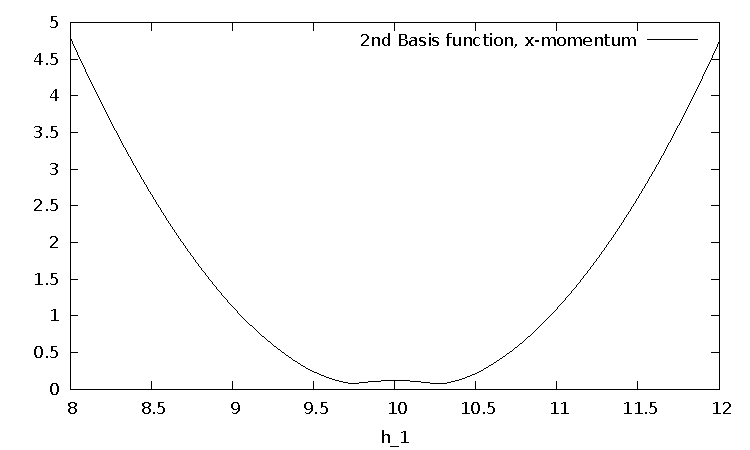
\includegraphics[scale=\zoomfactor]{{{magnitude_10_momentums/y_10.0_10.0_4.0_-2.0_2.0_-2.0_4.0_1.0f02}}}
  }
  \subfloat[Height values are $h_2=h_3=1000$. Variable $h_1$ ranges from 998 to 1002.] {
    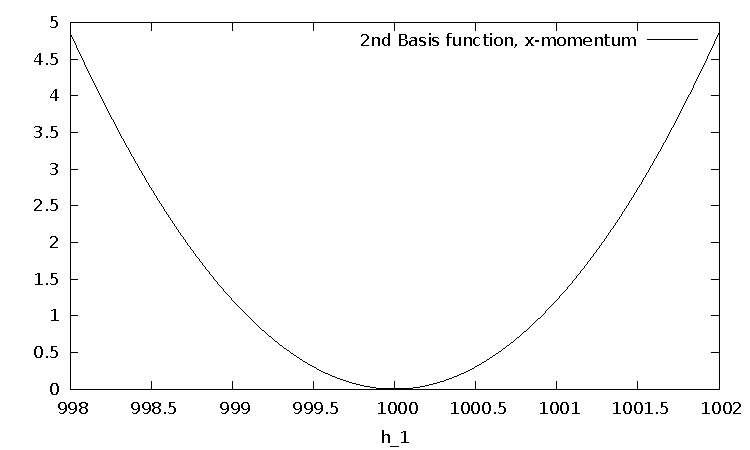
\includegraphics[scale=\zoomfactor]{{{magnitude_1000_momentums/y_1000.0_1000.0_4.0_-2.0_2.0_-2.0_4.0_1.0f02}}}
  }
\caption{Comparison of different orders of magnitude for non-standard momentum values $u_{x,1}=2, u_{x,2}= -2, u_{x,3}= 2, u_{y,1}= -2, u_{y,2}= 4, u_{y,3}=1$.}
\label{fig:magnitude_comp_momentums}
\end{figure}

%%% Local Variables:
%%% TeX-master: "../results.tex"
%%% End:
